\section{Schwingungen}
\subsection{Freie Schwingungen}
\subsubsection{Allgemein}

\formula{$ f = \dfrac{1}{T} $}
\formula{$ \omega = 2 \pi f $}
\formula{$ c = \dfrac{m g}{\Delta l} $}

\begin{center}
	\begin{minipage}{0.3\textwidth}
		Translationsbewegung / Linear \\
		\formula{$ F = m \cdot a $}
	\end{minipage}%%% to prevent a space
	\begin{minipage}{0.3\textwidth}
		Rotationsbewegung / Drehung \\
		\formula{$ M = J \cdot a $}
	\end{minipage}
\end{center}

\begin{center}
	\begin{minipage}{0.3\textwidth}
		\unit{$f$}{Frequenz}{$ \frac{1}{s} $} \\
		\unit{$c$}{Federkonstante}{$\frac{N}{m}$} \\
		\unit{$T$}{Periode}{$ s $} \\
	\end{minipage}%%% to prevent a space
	\begin{minipage}{0.3\textwidth}
		\unit{$m$}{Masse}{$ kg $} \\
		\unit{$g$}{Ardanziehung}{$ \frac{m}{s^2} $} \\
		\unit{$\Delta l$}{Federweg}{$ m $} \\
	\end{minipage}
\end{center}




\subsubsection{Harmonische Schwingung}

\begin{center}
	\begin{minipage}{0.25\textwidth}
		\formula{$ T = \dfrac{2 \pi}{\omega} $}
		\formula{$ y(t) = A \sin( \omega t + \varphi ) $}
		\formula{$ v(t) = \dot{y} = A \omega_0 \cos(\omega_0 t) $}
		\formula{$ a(t) = \ddot{y} = - A \omega_0 ^2 \sin(\omega_0 t) $} \\
		
		\unit{$A$}{Amplitude}{$1$} \\
		\unit{$\omega$}{Kreisfrequenz}{$\frac{1}{s}$} \\
		\unit{$t$}{Zeit}{$s$} \\
		\unit{$\varphi$}{Phasenverschiebung}{$rad$}
	\end{minipage}%%% to prevent a space
	\begin{minipage}{0.3\textwidth}
		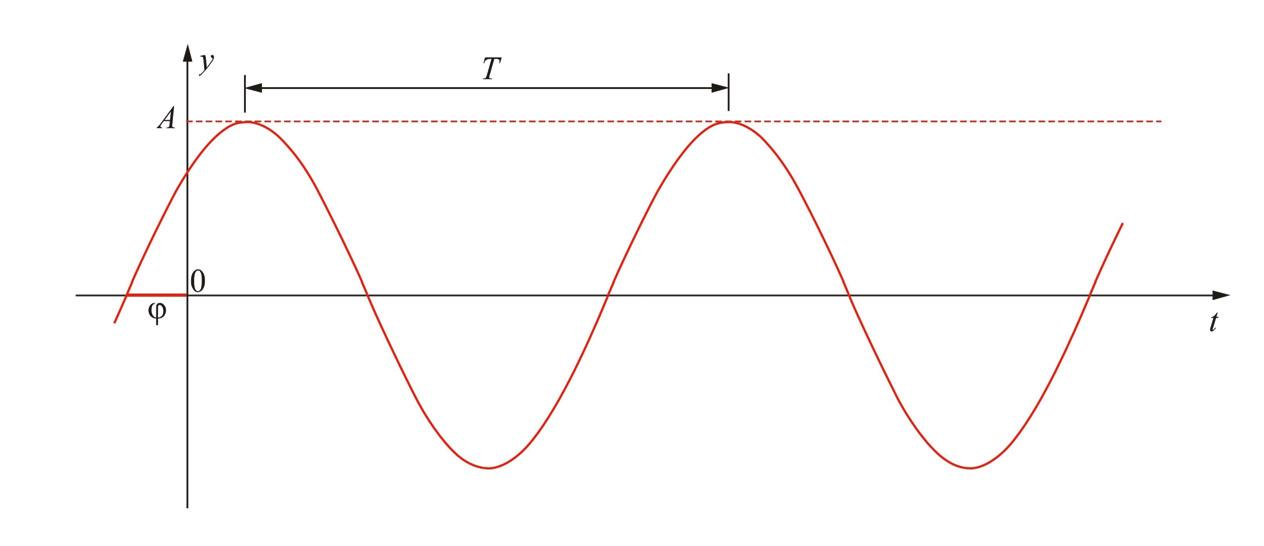
\includegraphics[height=3cm,keepaspectratio=true]{Images/harmonische_schwingung.png}
	\end{minipage}
\end{center}



\subsubsection{Federpendel}

\begin{center}
	\begin{minipage}{0.2\textwidth}
		\formula{$ F_1 = - F_{10} - c_1 \cdot y $}
		\formula{$ F_2 = F_{20} - c_2 \cdot y = F_0 - c \cdot y $}
		\formula{$ F_{RES} = -c \cdot y = F_1 + F_2 $}
		\formula{$ T = 2 \pi \sqrt{\dfrac{m}{c}} = \dfrac{2 \pi}{\omega_0} $}
		\formula{$ T = 2 \pi \sqrt{\dfrac{m + \dfrac{m_F}{3}}{c}} $)}
	\end{minipage}%%% to prevent a space
	\begin{minipage}{0.3\textwidth}
		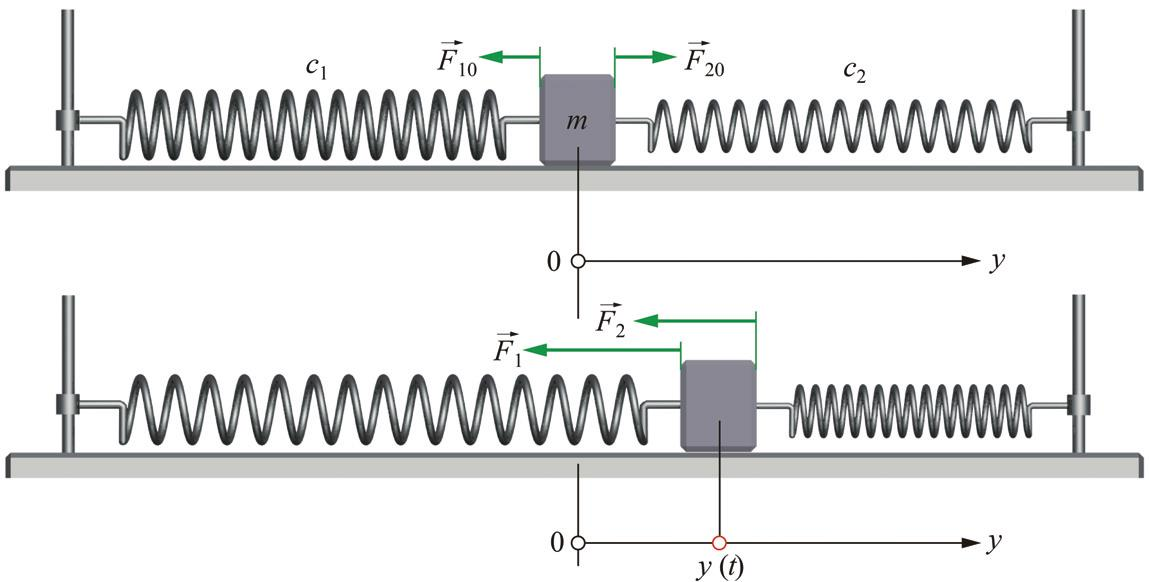
\includegraphics[height=4cm,keepaspectratio=true]{Images/federpendel.png}
	\end{minipage}
\end{center}

\formula{$ a(t) = - \left( \dfrac{c}{m} \right) y $}
\formula{$ y(t) = A \sin(\omega_0 t + \varphi) $}
\formula{$ \omega_0 = \sqrt{\dfrac{c}{m}} $}
\formula{$ m \ddot{y} + c y = 0 $}

\begin{center}
	\begin{minipage}{0.3\textwidth}
		\unit{$F_x$}{Kraft}{$N$} \\
		\unit{$T$}{Periode}{$s$} \\
		\unit{$a$}{Beschlaunigung}{$\frac{m}{s^2}$} \\
		\unit{$c$}{Federkonstante}{$\frac{N}{m}$} \\
		\unit{$m$}{Bewegte Masse}{$kg$}
	\end{minipage}%%% to prevent a space
	\begin{minipage}{0.3\textwidth}
		\unit{$m_F$}{Federmasse}{$kg$} \\
		\unit{$t$}{Zeit}{$sekunden$} \\
		\unit{$y$}{Auslenkung}{$m$} \\
		\unit{$\omega$}{Kreisfrequenz}{$\frac{1}{s}$} \\
		\unit{$\varphi$}{Nullphasenwinkel}{$rad$}
	\end{minipage}
\end{center}





\subsubsection{Drehpendel (Torsionspendel)}

\begin{center}
	\begin{minipage}{0.3\textwidth}
		\formula{$M = -c \varphi(t)$}
		\formula{$J = J_s + 2 m l^2$}
		\formula{$J \cdot \ddot{y} + c \cdot \varphi = 0$}
		\formula{$\omega = \sqrt{\dfrac{c}{J}}$}
		\formula{$T = 2 \pi \sqrt{\dfrac{J}{c}}$}
	\end{minipage}%%% to prevent a space
	\begin{minipage}{0.3\textwidth}
		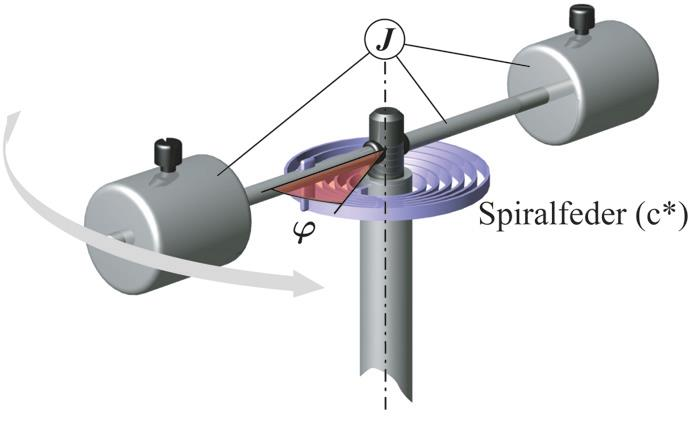
\includegraphics[height=3cm,keepaspectratio=true]{Images/drehpendel.png}
	\end{minipage}
\end{center}
\begin{center}
	\begin{minipage}{0.3\textwidth}
		\unit{$J$}{Massenträgheitmoment}{$\frac{kg}{m^2}$} \\
		\unit{$M$}{Drehmoment}{$N m$} \\
		\unit{$T$}{Periode}{$s$}
	\end{minipage}%%% to prevent a space
	\begin{minipage}{0.3\textwidth}
		\unit{$c$}{Federkonstant}{$\frac{N}{m}$} \\
		\unit{$y$}{Auslemkung}{$m$} \\
		\unit{$\omega$}{Kreisfrequenz}{$\frac{1}{s}$} \\
		\unit{$\varphi$}{Nullphasenwinkel}{$rad$}	
	\end{minipage}
\end{center}






\subsubsection{Schwerependel Mathematisch}
\begin{center}
	\begin{minipage}{0.3\textwidth}
		\formula{$M = l \cdot m \cdot g \cdot \sin(\varphi)$}
		\formula{$J = J_s + m \cdot l^2 = 0 + m \cdot l^2$}
		\formula{$T = 2 \pi \sqrt{\dfrac{l}{g}}$}
		\formula{$\omega_0 = \sqrt{\dfrac{g}{l}}$}
		\formula{$l \ddot{y} + g \sin(\varphi) = 0$}
		\formula{$l \ddot{y} + g \varphi = 0$}
	\end{minipage}%%% to prevent a space
	\begin{minipage}{0.3\textwidth}
		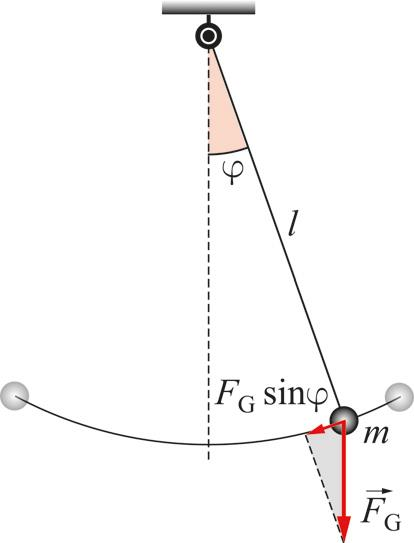
\includegraphics[height=4cm,keepaspectratio=true]{Images/schwerependel_mathematisch.png}
	\end{minipage}
\end{center}

\begin{center}
	\begin{minipage}{0.3\textwidth}
		\unit{$J$}{Massenträgheitmoment}{$\frac{kg}{m^2}$} \\
		\unit{$M$}{Drehmoment}{$N m$} \\
		\unit{$T$}{Periode}{$s$} \\
		\unit{$g$}{Erdbeschleunigung}{$\frac{m}{s^2}$}
	\end{minipage}%%% to prevent a space
	\begin{minipage}{0.3\textwidth}
		\unit{$l$}{Pendellänge}{$m$} \\
		\unit{$y$}{Auslemkung}{$m$} \\
		\unit{$\omega$}{Kreisfrequenz}{$\frac{1}{s}$} \\
		\unit{$\varphi$}{Winkel}{$rad$}
	\end{minipage}
\end{center}




\subsubsection{Schwerependel Physikalisch}
\begin{center}
	\begin{minipage}{0.3\textwidth}
		\formula{$T = 2 \pi \sqrt{\dfrac{J_A}{m \cdot g \cdot a}} =
			2 \pi \sqrt{\dfrac{J_S + m a^2}{m \cdot g \cdot a}} $}
		\formula{$\omega_0 = \sqrt{\dfrac{m \cdot g \cdot a}{J_A}}$}
		\formula{$l^* = \dfrac{J_A}{m a}$}
		\formula{$J_A \ddot{\varphi} = m g a \sin(\varphi) = 0 $}
		\formula{$J_A = J_S + m a^2$}
		\formula{$\omega_{max} = \sqrt{\dfrac{g}{2} \sqrt{\dfrac{m}{J_S}}}$}
		
	\end{minipage}%%% to prevent a space
	\begin{minipage}{0.3\textwidth}
		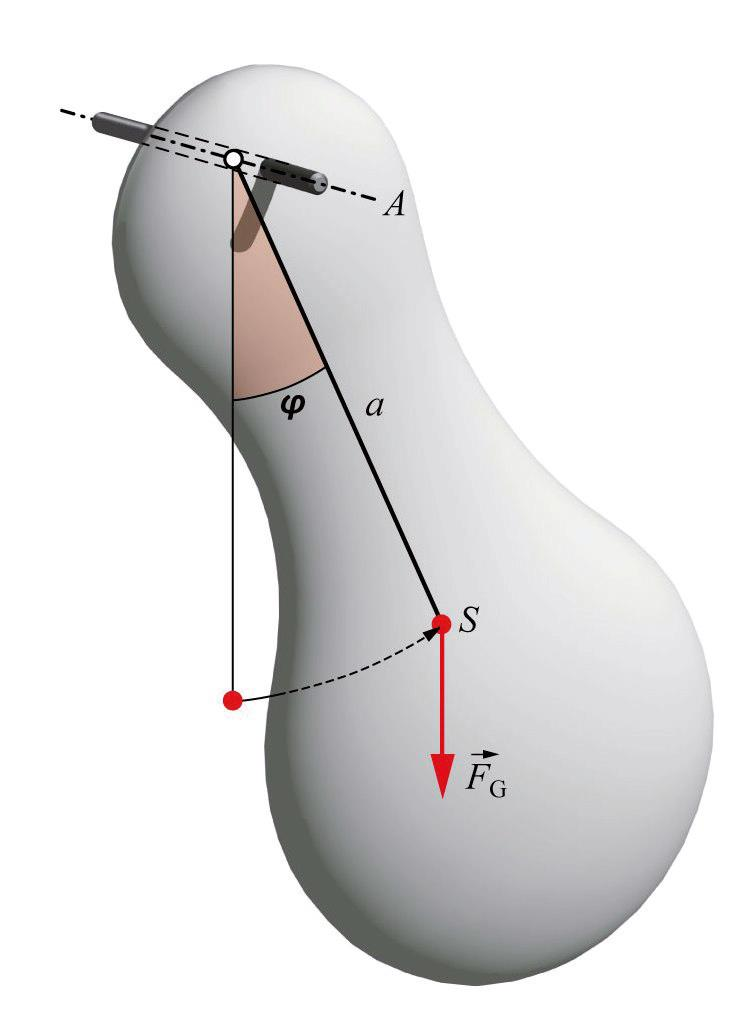
\includegraphics[height=4cm,keepaspectratio=true]{Images/schwerependel_physikalisch.png}
	\end{minipage}
\end{center}

\begin{center}
	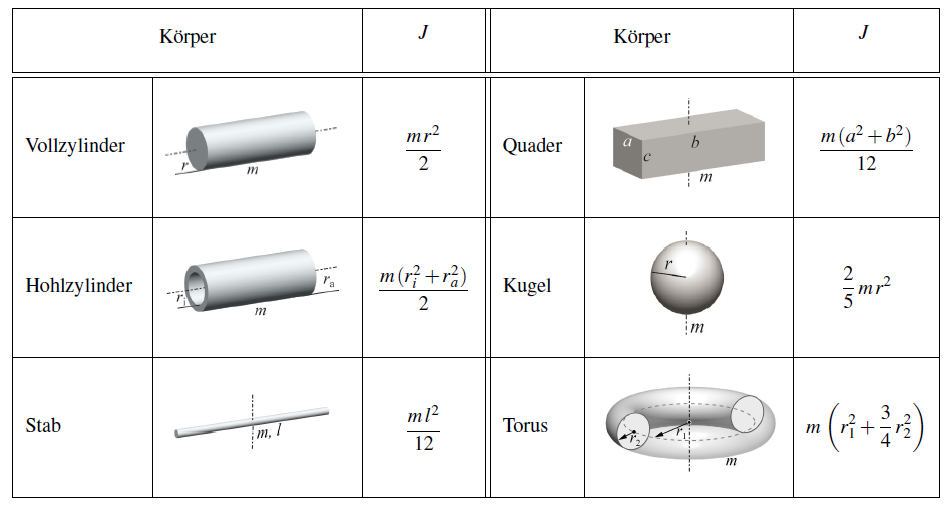
\includegraphics[height=7cm,keepaspectratio=true]{Images/traegheitsmomente.png}
\end{center}
\begin{center}
	\begin{minipage}{0.3\textwidth}
		\unit{$J_A$}{Massenträgheit bez. A-Achse}{$kg \cdot m^2$} \\
		\unit{$J_S$}{Massenträgheit bez. Achse $\parallel$ a}{$kg \cdot m^2$} \\
		\unit{$T$}{Periode}{$s$} \\
		\unit{$a$}{Abstand zum Schwerpunkt S}{$m$} \\
	\end{minipage}%%% to prevent a space
	\begin{minipage}{0.3\textwidth}
		\unit{$g$}{Erdbeschleunigung}{$\frac{m}{s^2}$} \\
		\unit{$m$}{Masse}{$kg$} \\
		\unit{$l^*$}{Reduzierte Pendellänge}{$m$} \\
		\unit{$\omega_0$}{Kreisfrequenz}{$\frac{1}{s}$} \\
	\end{minipage}
\end{center}




\subsubsection{Perkussionszentrum}
\begin{center}
	\begin{minipage}{0.3\textwidth}
		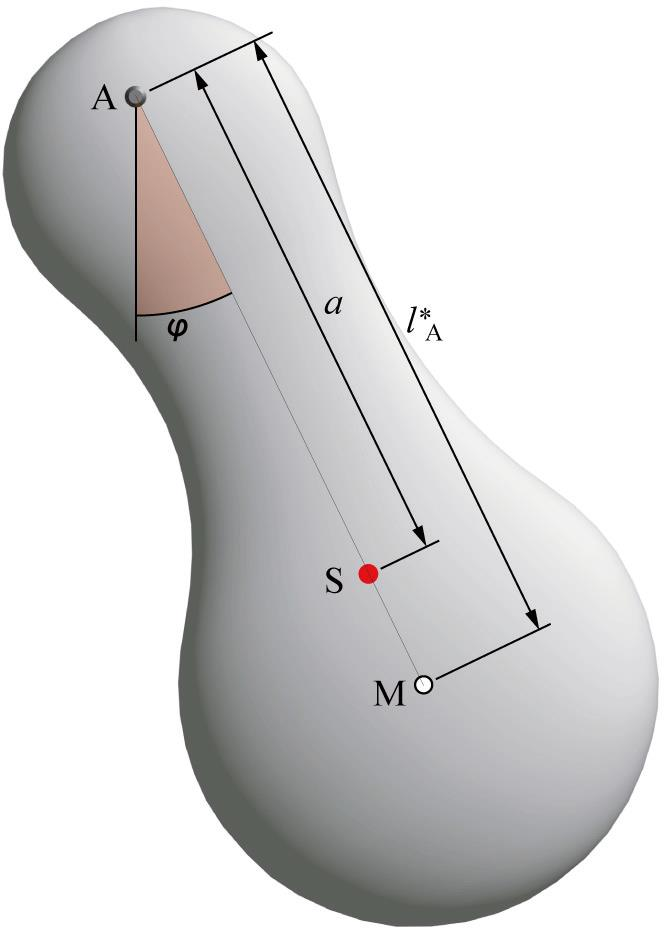
\includegraphics[height=5cm,keepaspectratio=true]{Images/schwerependel_perkussionszentrum.png}
	\end{minipage}%%% to prevent a space
	\begin{minipage}{0.3\textwidth}
		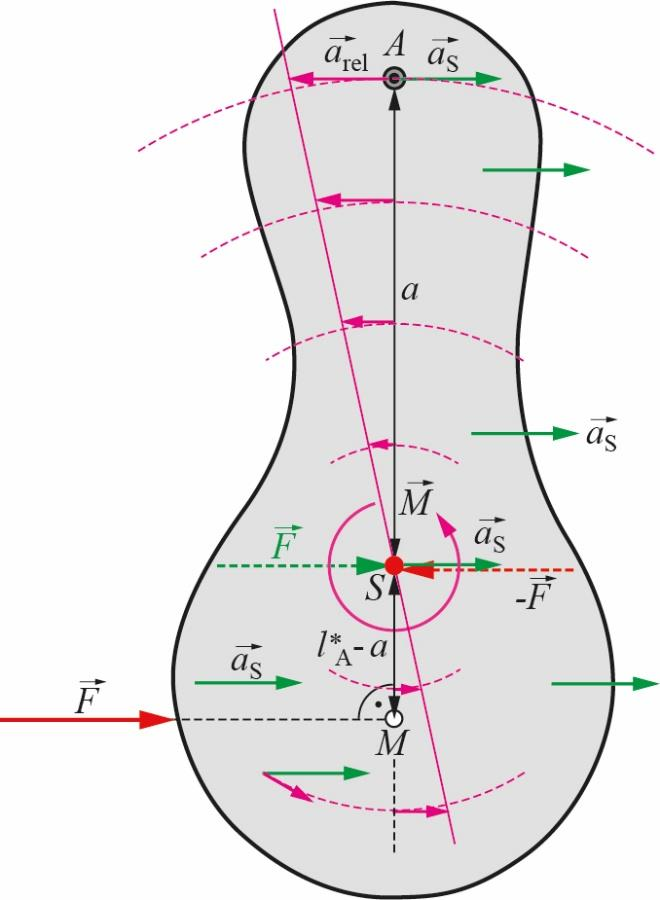
\includegraphics[height=5cm,keepaspectratio=true]{Images/perkussionszentrum.png}
	\end{minipage}
\end{center}




\subsubsection{Energie}
\begin{center}
	\begin{minipage}{0.2\textwidth}
		\formula{$E_{ges} = \frac{1}{2} c A^2 = E_{pot} + E_{kin}$} \\
		\formula{$E_{pot} = \frac{1}{2} c A^2 \cos^2(\omega t + \varphi)$} \\
		\formula{$E_{kin} = \frac{1}{2} c A^2 \sin^2(\omega t + \varphi)$} \\
		
		\unit{$E_{xyz}$}{Energie}{$J$} \\
		\unit{$A$}{Amplitude}{$m$} \\
		\unit{$c$}{Federkonstante}{$\frac{N}{m}$} \\
		\unit{$t$}{Zeit}{$s$} \\
		\unit{$\omega$}{Kreisfrequenz}{$\frac{1}{s}$}
	\end{minipage}%%% to prevent a space
	\begin{minipage}{0.3\textwidth}
		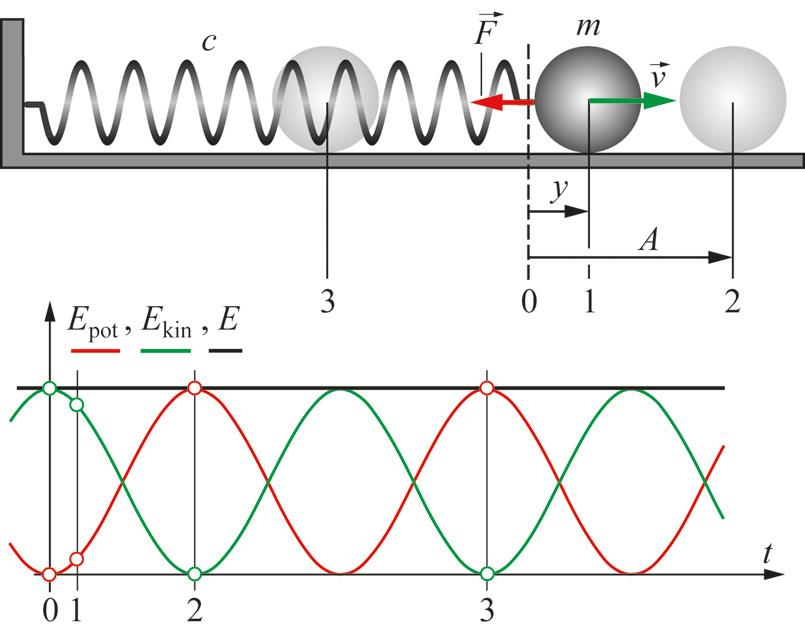
\includegraphics[height=4.5cm,keepaspectratio=true]{Images/schwingung_energie.png}
	\end{minipage}
\end{center}




\subsubsection{Gedämpfte Schwingung}
\begin{center}
	\begin{minipage}{0.2\textwidth}
		\formula{$F_G = m g$}
		\formula{$F_F = -c y$}
		\formula{$F_D = -b \dot{y}$}
		\formula{$m \ddot{y} + b \dot{y} + c y = 0$}
		\formula{$y = A e^{- \delta t} \sin(\omega_d t + \varphi_0)$}
		\formula{$\delta = \dfrac{b}{2 m}$}
		\formula{$\varLambda = \delta T$}
		\formula{$\varLambda = \ln \left(  \frac{A_n}{A_{n+1}} \right) $}
		\formula{$D = \dfrac{\delta}{\omega_0}$}
		\formula{$\dfrac{A_n}{A_{n+1}} = e^{\delta T}$}
		\formula{$m \ddot{y} = F_{Res} = F_F - F_G + F_D$}
	\end{minipage}%%% to prevent a space
	\begin{minipage}{0.3\textwidth}
		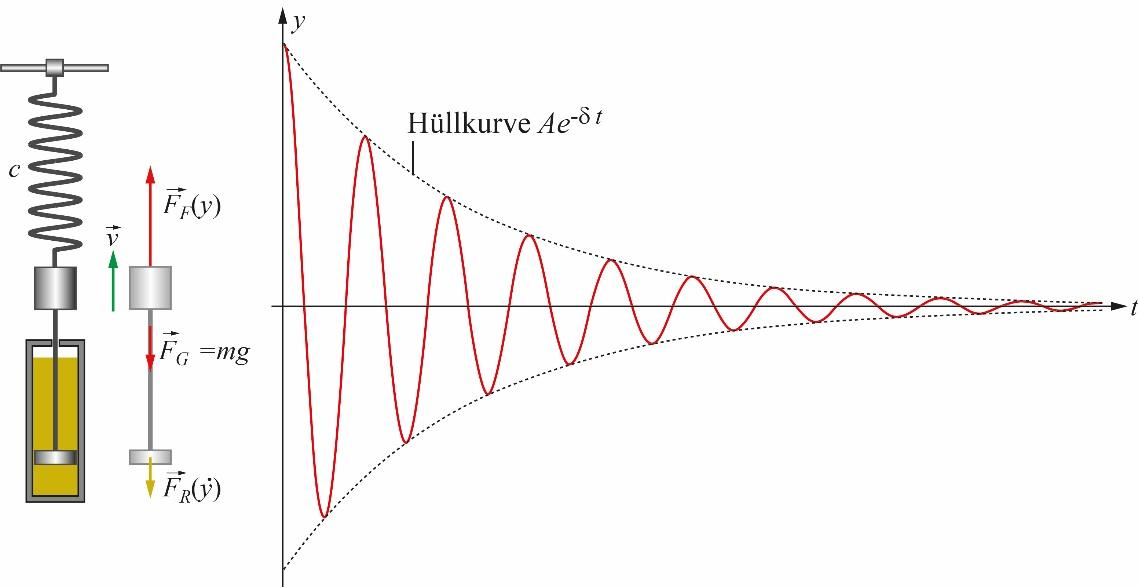
\includegraphics[height=4.5cm,keepaspectratio=true]{Images/gedaempfte_schwingung.png}
	\end{minipage}
\end{center}
\begin{center}
	\begin{minipage}{0.3\textwidth}
		\unit{$A$}{Amplitude}{$m$} \\
		\unit{$D$}{Dämpfungsgrad}{$1$} \\
		\unit{$F_G$}{Gewichtskraft}{$N$} \\
		\unit{$F_F$}{Federkraft}{$N$} \\
		\unit{$F_D$}{Dämpfungskraft}{$N$} \\
		\unit{$T$}{Periode}{$s$} \\
		\unit{$b$}{Dämpfungskonstante}{$1$}
	\end{minipage}%%% to prevent a space
	\begin{minipage}{0.3\textwidth}
		\unit{$c$}{Federkonstante}{$\frac{N}{m}$} \\
		\unit{$m$}{Masse}{$kg$} \\
		\unit{$y$}{Auslenkung}{$m$} \\
		\unit{$\delta$}{Abklingkonstante}{$1$} \\
		\unit{$\varphi$}{Nullphasenwinkel}{$rad$} \\
		\unit{$\omega$}{Kreisfrequenz}{$\frac{1}{s}$} \\
		\unit{$\varLambda$}{log. Dekrement}{$1$}
	\end{minipage}
\end{center}

\subsection{Fremderregte Schwingung}
\textbf{Formelsammlung 22.1.6 p.574}
\subsubsection{Krafterregung und Federkrafterregung}
\begin{center}
	\begin{minipage}{0.3\textwidth}
		\formula{$m \ddot{y} + b \dot{y} + c y = c u_0 \sin(\omega t)$}
		\formula{$\omega_r = \omega_0 \sqrt{1 - 2 D^2}$}
		\formula{$A = \dfrac{c u_0}{m \sqrt{(\omega^2_0 - \omega^2)^2 + (2 D \omega_0 \omega)^2}}$}
		\formula{$\omega_d = \sqrt{\omega^2_0 - \delta^2}$}
		\formula{$\varphi = \arctan \dfrac{2 D \omega_0 \omega}{\omega^2_0 - \omega^2}$}
		\formula{$A_r = \dfrac{u_0}{2 D \sqrt{1 - D^2}}$}
		\formula{$V = \dfrac{1}{\sqrt{(1 - \eta^2)^2 + (2 D \eta)^2}}$}
		\formula{$D = \dfrac{\delta}{\omega_0}$}
	\end{minipage}%%% to prevent a space
	\begin{minipage}{0.2\textwidth}
		\begin{center}
			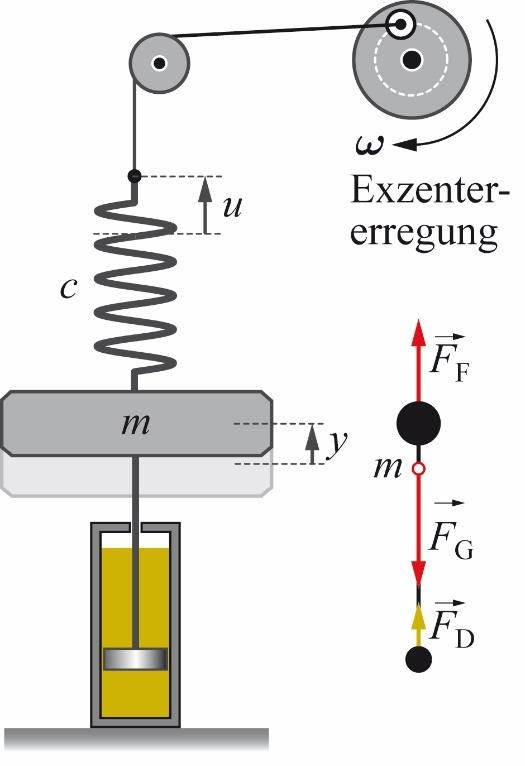
\includegraphics[height=4cm,keepaspectratio=true]{Images/krafterregung_a.png}
			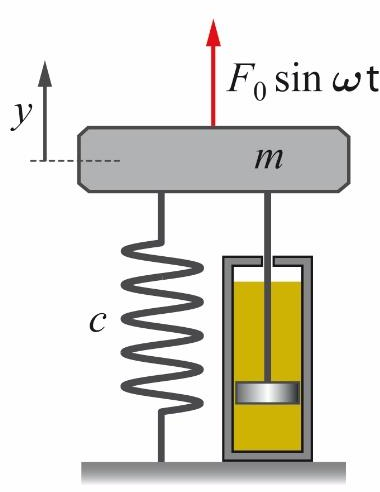
\includegraphics[height=3cm,keepaspectratio=true]{Images/krafterregung_b.png}
		\end{center}
	\end{minipage}
\end{center}

\unit{$\omega$}{Kreisfrequenz der Störung}{$\frac{rad}{s}$} \\
\unit{$\omega_0$}{Kreisfrequenz der ungedämpften Schwingung}{$\frac{rad}{s}$} \\
\unit{$\omega_d$}{Kreisfrequenz der gedämpften Schwingung}{$\frac{rad}{s}$} \\
\unit{$\omega_r$}{Resonanzkreisfrequenz}{$\frac{rad}{s}$} \\
\unit{$\delta$}{Abklingkonstante}{$\frac{1}{s}$} \\
\unit{$\eta$}{dimensionslose Frequenz}{$1$} \\
\unit{$A$}{Amplitude}{$m$} \\
\unit{$A_r$}{Resonanzamplitude}{$m$} \\
\unit{$D$}{Dämpfungsgrad}{$1$} \\
\unit{$V$}{Vergrösserungsfunktion}{$?$} \\

\subsubsection{Indirekte Federkrafterregung}
\formula{$m \ddot{y} + b \dot{y} + c y = c_2 u_0 \sin(\omega t)$}
\formula{$A = \dfrac{c_2}{c} \dfrac{c u_0}{m \sqrt{(\omega^2_0 - \omega^2)^2 + (2 D \omega_0 \omega)^2}}$}
\formula{$\varphi = \arctan \dfrac{2 D \omega_0 \omega}{\omega^2_0 - \omega^2}$}
\formula{$\omega_r = \omega_0 \sqrt{1 - 2 D^2}$}
\formula{$A_r = \dfrac{u_0}{2 D \sqrt{1 - D^2}}$}
\formula{$V = \dfrac{c_2}{c} \dfrac{1}{\sqrt{(1 - \eta^2)^2 + (2 D \eta)^2}}$}

\unit{$\omega$}{Kreisfrequenz der Störung}{$\frac{rad}{s}$} \\
\unit{$\omega_0$}{Kreisfrequenz der ungedämpften Schwingung}{$\frac{rad}{s}$} \\
\unit{$\omega_r$}{Resonanzkreisfrequenz}{$\frac{rad}{s}$} \\
\unit{$\eta$}{dimensionslose Frequenz}{$1$} \\
\unit{$\varphi$}{Phase}{$rad$} \\
\unit{$A$}{Amplitude}{$m$} \\
\unit{$A_r$}{Resonanzamplitude}{$m$} \\
\unit{$D$}{Dämpfungsgrad}{$1$} \\
\unit{$V$}{Vergrösserungsfunktion}{$?$} \\

\subsubsection{Dämpferregung}
\begin{center}
	\begin{minipage}{0.4\textwidth}
		\formula{$m \ddot{y} + b \dot{y} + c y = b \omega u_0 \sin(\omega t + \dfrac{\pi}{2})$}
		\formula{$V = \dfrac{2 D \eta}{\sqrt{(1 - \eta^2)^2 + (2 D \eta)^2}}$}
		\formula{$A = \dfrac{b \omega u_0}{m \sqrt{(\omega^2_0 - \omega^2)^2 + (2 D \omega_0 \omega)^2}}$}
		\formula{$\varphi = \arctan \dfrac{2 D \omega_0 \omega}{\omega^2_0 - \omega^2} - \dfrac{\pi}{2}$}
		\formula{$\omega_r = \omega_0$}
		\formula{$A_r = u_0$}
		\formula{$V = \dfrac{2 D \eta}{\sqrt{(1 - \eta^2)^2 + (2 D \eta)^2}}$}
	\end{minipage}%%% to prevent a space
	\begin{minipage}{0.1\textwidth}
		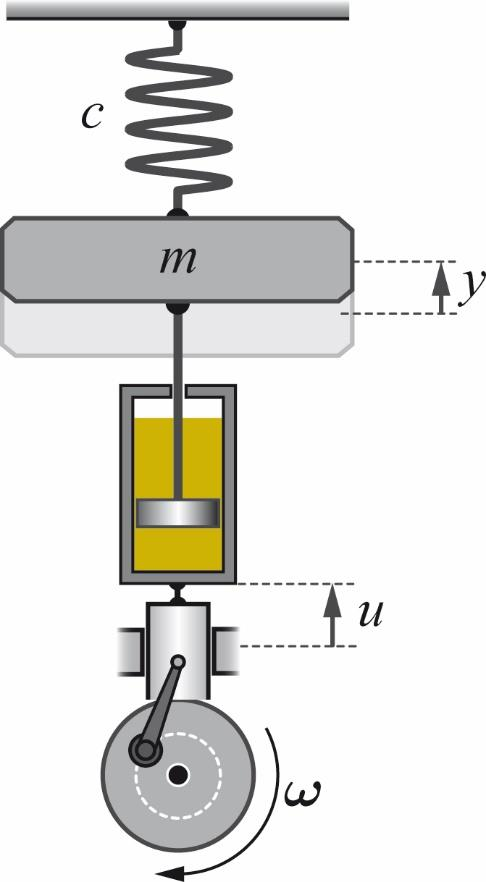
\includegraphics[height=3cm,center,keepaspectratio=true]{Images/daempferregung.png}
	\end{minipage}
\end{center}

\unit{$\omega$}{Kreisfrequenz der Störung}{$\frac{rad}{s}$} \\
\unit{$\omega_0$}{Kreisfrequenz der ungedämpften Schwingung}{$\frac{rad}{s}$} \\
\unit{$\omega_r$}{Resonanzkreisfrequenz}{$\frac{rad}{s}$} \\
\unit{$\eta$}{dimensionslose Frequenz}{$1$} \\
\unit{$\varphi$}{Phase}{$rad$} \\
\unit{$A$}{Amplitude}{$m$} \\
\unit{$A_r$}{Resonanzamplitude}{$m$} \\
\unit{$D$}{Dämpfungsgrad}{$1$} \\
\unit{$V$}{Vergrösserungsfunktion}{$?$} \\

\subsubsection{Stützerregung}
\begin{center}
	\begin{minipage}{0.4\textwidth}
		\formula{$m \ddot{y} + b \dot{y} + c y = c u_0 \sin(\omega t + b \omega) u_0 \cos(\omega t)$}
		\formula{$m \ddot{q} + b \dot{q} + c q = m \omega^2 u_0 \sin(\omega t)$}
		\formula{$A = \dfrac{\omega^2 u_0}{\sqrt{(\omega^2_0 - \omega^2)^2 + (2 D \omega_0 \omega)^2}}$}
		\formula{$\varphi = \arctan \left(  \dfrac{2 D \omega_0 \omega}{\omega^2_0 - \omega^2} \right) - \pi$}
		\formula{$\omega_r = \dfrac{\omega_0}{\sqrt{1 - 2 D^2}}$}
		\formula{$A_r = \dfrac{u_0}{2 D \sqrt{1 - D^2}}$}
		\formula{$V = \dfrac{\eta^2}{\sqrt{(1 - \eta^2)^2 + (2 D \eta)^2}}$}
	\end{minipage}%%% to prevent a space
	\begin{minipage}{0.1\textwidth}
	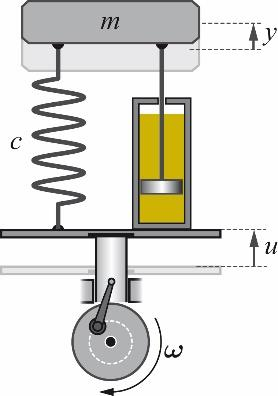
\includegraphics[height=3cm,center,keepaspectratio=true]{Images/stuezerregung.png}
	\end{minipage}
\end{center}

\unit{$\omega$}{Kreisfrequenz der Störung}{$\frac{rad}{s}$} \\
\unit{$\omega_0$}{Kreisfrequenz der ungedämpften Schwingung}{$\frac{rad}{s}$} \\
\unit{$\omega_r$}{Resonanzkreisfrequenz}{$\frac{rad}{s}$} \\
\unit{$\eta$}{dimensionslose Frequenz}{$1$} \\
\unit{$\varphi$}{Phase}{$rad$} \\
\unit{$A$}{Amplitude}{$m$} \\
\unit{$A_r$}{Resonanzamplitude}{$m$} \\
\unit{$D$}{Dämpfungsgrad}{$1$} \\
\unit{$V$}{Vergrösserungsfunktion}{$?$} \\

\subsubsection{Unwuchterregung}
\begin{center}
	\begin{minipage}{0.25\textwidth}
		\formula{$m \ddot{y} + b \dot{y} + c y = m_R e \omega \sin(\omega t)$}
		\formula{$A = \dfrac{m_R e \omega^2}{\sqrt{(\omega^2_0 - \omega^2)^2 + (2 D \omega_0 \omega)^2}}$}
		\formula{$\varphi = \arctan \dfrac{2 D \omega_0 \omega}{\omega^2_0 - \omega^2}$}
		\formula{$\omega_r = \dfrac{\omega_0}{\sqrt{1 - 2 D^2}}$}
		\formula{$A_r = \dfrac{m_R}{m} = \dfrac{e}{2 D \sqrt{1 - D^2}}$}
		\formula{$\dfrac{F_{B0}}{F_0} = \sqrt{\dfrac{1 + 4 D^2 \eta^2}{(1 - \eta^2)^2 + 4 D^2 \eta^2}}$}
	\end{minipage}%%% to prevent a space
	\begin{minipage}{0.25\textwidth}
		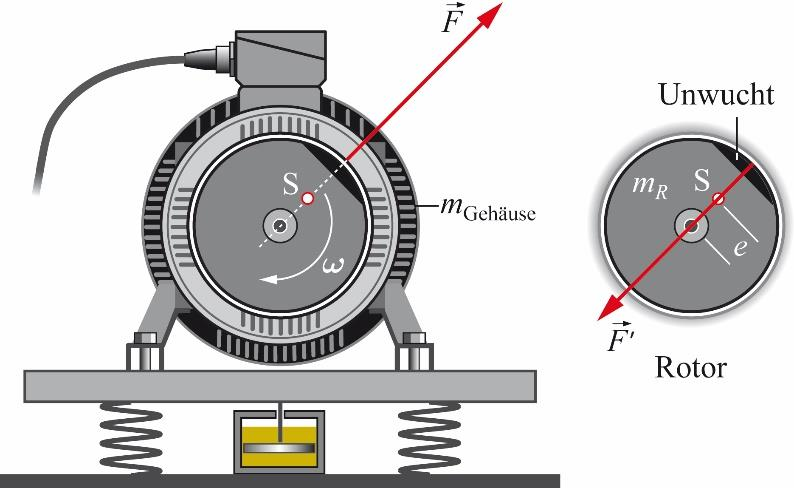
\includegraphics[height=3cm,center,keepaspectratio=true]{Images/unwuchterregung.png}
		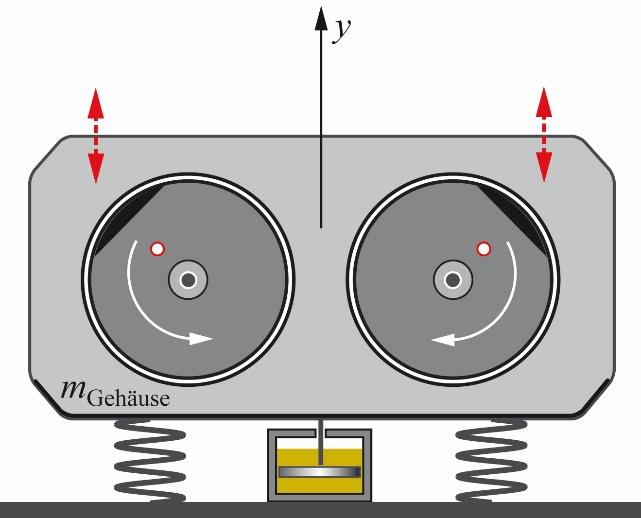
\includegraphics[height=3cm,center,keepaspectratio=true]{Images/unwuchterregung_doppelt.png}
	\end{minipage}
\end{center}

\unit{$\omega$}{Kreisfrequenz der Störung}{$\frac{rad}{s}$} \\
\unit{$\omega_0$}{Kreisfrequenz der ungedämpften Schwingung}{$\frac{rad}{s}$} \\
\unit{$\omega_r$}{Resonanzkreisfrequenz}{$\frac{rad}{s}$} \\
\unit{$\eta$}{dimensionslose Frequenz}{$1$} \\
\unit{$\varphi$}{Phase}{$rad$} \\
\unit{$A$}{Amplitude}{$m$} \\
\unit{$A_r$}{Resonanzamplitude}{$m$} \\
\unit{$D$}{Dämpfungsgrad}{$1$} \\

\subsubsection{Serienschwingkreis}
\formula{$L \ddot{I} + R_s \dot{I} + \dfrac{1}{C} I = \omega U_0 \sin(\omega t + \dfrac{\pi}{2})$}
\formula{$I_0 = \dfrac{\omega U_0}{L \sqrt{(\omega^2_0 - \omega^2)^2 + (2 D \omega_0 \omega)^2}}$}
\formula{$\varphi = \arctan \left( \dfrac{2 D \omega_0 \omega}{\omega^2_0 - \omega^2} \right) - \dfrac{\pi}{2}$}
\formula{$\omega_r = \omega_0$}
\formula{$I_{0r} = \dfrac{U_0}{R_s}$}
\formula{$V = \dfrac{\eta^2}{\sqrt{(1 - \eta^2)^2 + (2 D \eta)^2}}$}
\formula{$\varphi_U = \arctan \left( \dfrac{2 D \eta}{1 - \eta^2} \right) - \pi$}
\formula{$D = \dfrac{R_s}{2} \sqrt{\dfrac{C}{L}}$}

\subsubsection{Parallelschwingkreis}
\formula{$L \ddot{U} + R_s \dot{U} + \dfrac{1}{L} U = \omega I_0 \sin(\omega t + \dfrac{\pi}{2})$}
\formula{$U_0 = \dfrac{\omega I_0}{C \sqrt{(\omega^2_0 - \omega^2)^2 + (2 D \omega_0 \omega)^2}}$}
\formula{$\varphi = \arctan \left( \dfrac{2 D \omega_0 \omega}{\omega^2_0 - \omega^2} \right) - \dfrac{\pi}{2}$}
\formula{$\omega_r = \omega_0$}
\formula{$U_{0r} = R_p I_0$}
\formula{$V = \dfrac{1}{\sqrt{(1 - \eta^2)^2 + (2 D \eta)^2}}$}
\formula{$\varphi_I = \arctan \left( \dfrac{2 D \eta}{1 - \eta^2} \right)$}
\formula{$D = \dfrac{1}{2 R_p} \sqrt{\dfrac{L}{C}}$}









